\section{Lecture 13(?)}
% Bruno is back

The goal is to obtain 
\begin{equation}
    \begin{split}
        dX_t= b_t(X_t) dt + \sigma (X_t)\dif B_t\\
        X_t = X_0 + \int_0^t b_s ds + \int_0^t \sigma_s \dif B_s
    \end{split}
\end{equation}
$h(B_t)=: X_t$ what happens if we differentiate? We already did this calculation explicitly, and we found all the differentiation rules, at the end 
\begin{equation*}
	X_t -X_0 = \int_0^t [\partial_t h(s, B_s)+ \frac{1}{2} \partial^2_x h(s, B_0)]ds + \int_0^t \partial_x  h(s, B_s) \dif B_s
\end{equation*}
and this is the Ito formula. We didn't prove this one but it is the same as the following 
\begin{equation*}
	X_t-X_0 = \int_0^t h''(B_s)ds + \frac{1}{2}\int_0^t h'(B_s)\dif B_s
\end{equation*}
\begin{Th}
	Let $h: \mR_+ \times \mR \to \mR $ be $C'$ in $h(\cdot, x)$ and $C^2$ in  $h(t,\cdot)$ . Define $X_t:=h(t,B_t)$. Then $X_t$ is an Ito process and 
	\begin{equation*}
			X_t -X_0 = \int_0^t [\partial_t h(s, B_s)+ \partial^2_x h(s, B_s)]ds + \int_0^t \partial_x  h(s, B_s) \dif B_s 
	\end{equation*}
\end{Th}
\begin{proof}
	not done in class, in toaldo's notes 
\end{proof}
\begin{Th}
	Let $(X_t)_{t\geq 0}$ be an Ito process with drift $b_t$ and diffusion $\sigma_t$. Let $h: \mR_+ \times \mR \to \mR$ such that $h$ is in $\mC'$ in $h(\cdot, x)$ and $C^2$ in  $h(t,\cdot)$. Let $Y_t:= h(t, X_t)$. Then $Y_t$ is an Ito process and 
	\begin{equation*}
		Y_t -Y_0 = \int_0^t [\partial_t h(s, X_s)+ b_s \partial_x h(s, X_s)+ \frac{1}{2}\sigma^2 _s \partial^2_x h(s, X_s]ds + \int_0^t \sigma_s \partial_x  h(s, X_s) \dif B_s 
	\end{equation*}
\end{Th}
comment: \\
$b_s \partial_x h(s, X_s)$ in compact notation this will be non ha mei detto cosa sarebbe.
\begin{equation*}
	 dY_t = [\partial _t h(t,X_t) + \frac{1}{2}\sigma^2_t \partial_x^2h(t,X_t)]dt + \underbrace{b_t \partial_x h(t,X_t) dt + \sigma_t \partial :x b(t, X_t) \dif B_t}_{***}
\end{equation*}
forse ha scritto qualcos'altro in compact notation 
\begin{equation*}
	dX_t = b_t dt + \sigma_t \dif B_t =: \int_0^t \partial_x h(s, X_s) dX_s 
\end{equation*}
immagine we want to integrate not against BM but using an ito process, you will need to redo all the computation. Rebember that is just noise. 
so $***$ became 
\begin{equation*}
	dY_t = [\partial_t h(t,X_t)+ \frac{1}{2}\sigma_t^2 \partial^2_x ]+\partial_x h(s, X_s) dX_s  
\end{equation*}
Rules of differientiation:
\begin{equation*}
	\begin{split}
		dtdt=0 \hspace{2 cm} \dif B_t dt& = 0= dt\dif B_t \\
		(\dif B_t)^2&= dt
	\end{split}
\end{equation*}
Find a random process $(X_t){t\geq 0}$ satisfying 
\begin{equation*}
	\begin{cases}
		dX_t = \underbrace{b_t(X_t)dt }_{\text{Riemann}}+ \underbrace{\sigma_t (X_t)\dif B_t } _{Ito}\\
		X_0=x
	\end{cases}
\end{equation*}
\begin{Th}
	Let $T>0$ and suppose that there exist constant $C,D>0$ such that for every $t \in [0,T]$ the following condition hold:
	\begin{itemize}
		\item Lipschitz condition
		\begin{equation*}
			|b_t(x)-b_t(y)|+|\sigma_t(x)-\sigma_t(y)|\leq D|x-y|
		\end{equation*}
		\item linear growth condition \footnote{In reality this condition derive from the first one, bit the theorem is usually staten in this way. }
		\begin{equation*}
			|b_t(x)|+|\sigma_t(x)|\leq C(1+|x|)
		\end{equation*}
		
	\end{itemize}
	for any $x,y\in \mR$.\\
	Then there exists a unique random process $(X_t^x)_{t \in [0,T]}$ on the wiener space such that it is a solution of the SDE. Furthermore foto
	\begin{itemize}
		\item $\mE \int_0^t |X^x_s|^2 ds < + \infty$
		\item $[0,T]\ni t \ra X_t^x(\omega)$ is a.s. continuous
		\item $(X_t^x)_{t \in [0,T]}$ is adapted to $(\mathcal{F}_t)_{t \geq 0}$
	\end{itemize}
\end{Th}
the filtration is not necessary the natural it just need to be such that $X_t$ is a BM. the first 2 condition are progressively measurable $M^2$ . 
\begin{proof}
	In toaldo's notes but 
	\begin{remark} % o definizione  non siamo d'accordo
		\emph{Uniqueness:} Given two solutions $X_t^x$ and $Y_t^x$ 
		\begin{equation*}
			\mP(X_t^x = Y_t^x, \quad \forall t \in [0,T])=1
		\end{equation*}
		\emph{Existence:} picard approximation
	\end{remark}
	In class we will prove uniqueness. Suppose that there exist two solutions, $(X_t^x)_{t \in [0,T]}$ and $(Y_t^x)_{t \in [0,T]}$ then 
	\begin{enumerate}
		\item $X_t^x = Y_t^x$ a.s. $ \forall t in [0,T ]$
        \item $X_t^x = Y_t^x$ $ \forall t in [0,T ]$ a.s. 
	\end{enumerate}
 \begin{enumerate}
     \item 



     \item 
 \end{enumerate}
\end{proof}








\section{Lecture 14}
In the previous lecture we proved a result concerning the existence and the uniqueness of
\begin{equation*}
    dX_t = b_t(X_t) dt + \sigma_t(X_t) \dif B_t
\end{equation*}
Let us revise the heuristic discussion we already made at the beginning of the course. \\
The point is that the behavior of
\begin{equation*}
    dX_t = b_t(X_t) dt 
\end{equation*}
is a deterministic equation: $dX_t = X_{t+dt} - X_t$, once the current position is available, is known. \\
IMMAGINE \\
So the infinitesimal increment depends on the increment of time through a number which is dependent on the current position $X_t$. \\
To add randomness, we insert the second term, obtaining the initial differential equation: 
\begin{equation*}
    dX_t = b_t(X_t) dt + \sigma_t(X_t) \dif B_t
\end{equation*}
If we are in the current position and we want to understand what happens in the future, the only thing we need is ... 

The BM component actually cares only about $dt$, not the current position or time $t$. So this process is strongly Markovian. \\
Recall that there exist homogeneous and non-homogeneous processes. Heuristically, it means that the local evolution of the process at time $t$ does not depend on $t$. In the equation this means that if we want to have an homogeneous process we must avoid the dependence on $t$ of the functions $b_t$ and $\sigma_t$. \\

If we also want space-homogeneity, that is the behavior does not depend on the current position, $b$ and $\sigma$ are going to be just constant functions. \\
Therefore, with the two homogeneities, the local behavior does not depend on anything. \\
\begin{equation*}
    dX_t = b dt + \sigma \dif B_t
\end{equation*}
\begin{equation*}
    X_t = bt + \sigma B_t
\end{equation*}
\begin{DefBox}
    \begin{Def}
        A right-continuous process $(X_t)_{t \geq 0}$ on $(\Omega, \mathcal{F}, \mP)$, with $(\mathcal{F}_t)_{t \geq 0}$ is said to be a Markov process with respect to the filtration $\mathcal{F}_t$ is 
        \begin{equation*}
            \mE[u(X_t) | \mathcal{F}_s] = \mE[u(X_t)| X_s]
        \end{equation*}
        for all $t > s > 0$ and $u \in \mathcal{B}_b(\mR^d)$ (Borel bounded measurable function).
    \end{Def}
\end{DefBox}
It reduces to normal expected value in conditional probability if we consider the indicator $u = \mathbbm{1}_B, \quad B \in \mathcal{B}(\mR)$. 
\begin{ThBox}
    \begin{Th}
        The unique solution of the SDE is a Markov process with respect to $\mathcal{F}_t^B$. 
    \end{Th}
\end{ThBox}
\begin{ProofBox}
    \begin{proof}[Sketch of proof]
        Fix $t > s, s \geq 0$ and write the following SDE:
        \begin{equation*}
            X_t^{s,x} = x + \int_s^t (b(r,X_r^{s,x}) dr + \int_s^t \sigma(s,X_s^{s,x}) \dif B_s.
        \end{equation*}
        This is just the same SDE as above but with the additional inclusion of $s$.
        Even if the process does not start from $0$, this is not a problem. We just specify that $x$ is the spatial starting point and $s$ is the starting time. \\
        The previous SDE has unique solution
        \begin{equation*}
            (X_t^{s,x})_{t \geq s}
        \end{equation*}
        Fix $\xi \in \mR_+$
        \begin{equation*}
            X_t^{0,\xi} = \xi + \int_0^t b(r,X_r^{0,\xi}) dr + \int_0^t b(r,X_r^{0,\xi})\dif B_r
        \end{equation*}
        so
        \begin{equation*}
            X_t^{0,\xi}=X_n^{0,\xi}+\int_s^tb(r,X^{0,\xi}_r)\dif r+\int_{s}^{t}\sigma(r,X_r^{0,\xi})\dif B_r.
        \end{equation*}
        Now we use the uniqueness of the solution to get
        \begin{equation*}
        	X_t^{0,\xi}=X_t^{0,X_s^{0,\xi}}\qquad \text{a.s. }t\geq s.
        \end{equation*}
        Here the initial condition is in itself a random variable. Normally this should make us very uncomfortable, but for some reason Daddy Toaldo told us not to fret.
        The two assertions (equation e UNIQUENESS) allow us to define a functional of this form:
        \begin{equation*}
            X_t^{0,\xi} = \Phi(X_s^{0,\xi}, s, t, \omega).
        \end{equation*}
        This functional is measurable with respect to the filtration $\mathcal{G}_s := \sigma(B_r-B_s: t \geq s)$, which is generated by the BM. \\
        The random part of the previous equation is given by the presence of $\omega$, so we are dealing with an Ito integral. \\
        The independence of increments implies that
        \begin{equation*}
            \mathcal{G}_s \text{ is independent of } \mathcal{F}_s^B
        \end{equation*}
        \begin{equation*}
            \omega \mapsto \Phi(y,s,t,\omega)
        \end{equation*}
        is $\mathcal{G}_s$ - measurable. 
        %mi sono già rotta le palle 
        %FROZEN con sguardo spaventato e mani in alto
		Now take the following expectation for a function $u\in\mathcal{B}_b(\R)$:
		\begin{align*}
			&\ev{u(X_t^{0,\xi})|\mathcal{F}_s}\\
			=&\ev{u\left(\Phi\left(X_s^{0,\xi},s,t,\cdot\right)\right)\Big|\mathcal{F}_s}.
		\end{align*}
		Notice how we used ad $\cdot$ instead of $\omega$ because inside the expectation we effectively sum all the distribution mass up to $\omega$. We now
		need to state a lemma, which is equivalent to the Freezing Lemma (but it is more useful for our purposes)
        \begin{PropBox}
            \begin{Lemma}[Lemma A3 page 363, Schilling BM] 
            \end{Lemma}
        \end{PropBox}
        The basically tells us that 
        \begin{equation*}
        	\ev{u\left(\Phi\left(X_s^{0,\xi},s,t,\cdot\right)\right)\Big|\mathcal{F}_s}=\ev{u\left(\Phi(y,s,t,\cdot)\right)}\Big|_{y=X_s^{0,\xi}}
        \end{equation*}
        If we take the mapping $\omega\mapsto\Phi(y,s,t,\omega)$ then we know that it is $\mathcal{G}$-measurable. But if we look at the expectation then the dependence from $\omega$ has nothing to do with $\mathcal{F}_s$. $X_s^{0,\xi}$, on the other hand, \textit{is} dependent from $\mathcal{F}_t$.
        Since it is measurable (completely determined by the filtration), we can "freeze" it since it is a number, get an unconditioned expectation and move on with the proof. \\
        The dot in the third line stands for the function which acts to the last components and does not care about the first one (now called $y$) since the latter has been frozen. \\
        So now we can compute the expectation first using $y$ as a simple number and only after we plug in the random variable $X_s^{0,\xi}$ (which, remember, is the starting point). Now we get
        \begin{equation*}
        	\ev{u\left(X_t^{s,y}\right)}|_{y=X_s^{0,\xi}}.
        \end{equation*}
        This is not exactly the Markov statement, but we can get it nevertheless. Take
        \begin{align*}
        	\ev{\ev{u\left(X_t^{0,\xi}\right)|\mathcal{F}_s}|X_s^{0,\xi}}&=\ev{u\left(X_t^{0,\xi}|X_s^{0,\xi}\right)}\\
        	&=\ev{u\left(X_t^{s,y}\right)}\Big|_{y=X_s^{0,\xi}}\\
        	&=\ev{u(X_t^{0,\xi})|\mathcal{F}_s}
        \end{align*}
        o that we proved
        \begin{equation*}
        	\ev{u(X_t^{0,\xi})|\mathcal{F}_s}=\ev{u\left(X_t^{0,\xi}|X_s^{0,\xi}\right)}.
        \end{equation*}
    \end{proof}
\end{ProofBox}
Consider the family of measures, depending on $t,s$ and $x$ for $t \geq s$
\begin{equation*}
    \mP(X_t \in E | X_s=x) =: p(s,x;t,E)
\end{equation*}
These are called \textbf{transition probabilities of the Markov process} $(X_t)_{t \geq 0}$. If this family $p(s,x,t,\cdot)$ depends only on the distance between $s,t$ ($t-s$), then $X_t$ is said to be \textbf{homogeneous}. 
\begin{PropBox}
    \begin{Cor}
        If the coefficients of the SDE ($b,\sigma$) do not depend on time, then the solution (unique) is an homogeneous Markov process. 
    \end{Cor}
\end{PropBox}
If we take
\begin{equation*}
	\dif X_t=b(X_t)\dif t+\sigma(X_t)\dif B_t
\end{equation*}
as long as $b$ and $\sigma$ are Lipschitz continuous then $X_t$ is a homogeneous-time Markov process such that
\begin{equation*}
		\ev{u(X_t^{0,\xi})|\mathcal{F}_s}=\ev{u\left(X_t^{0,\xi}|X_s^{0,\xi}\right)}.
\end{equation*}
This means that we can ``translate'' the path:
\begin{figure}[H]
	\centering
	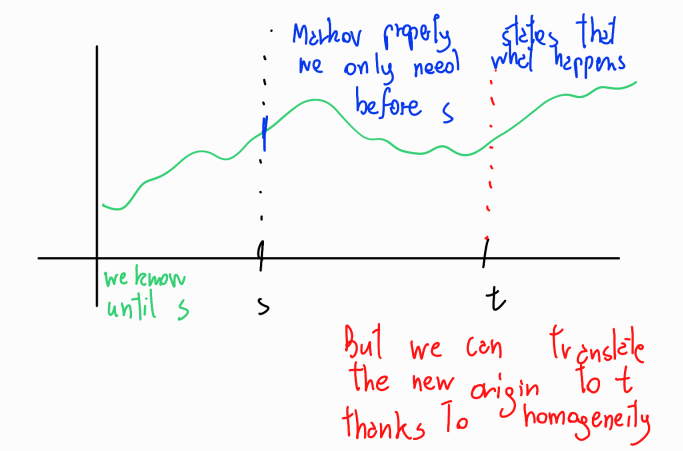
\includegraphics[width=0.7\linewidth]{screenshot001}
\end{figure}
Moreover, this means that
\begin{align*}
	\ev{u(X_t)|\mathcal{F}_s}&=\ev{u(X_t)|X)s}\\
	&=\mE^{X_s}\left[X_{t-s}\right]\\
	:&=\mE^{x}\left[u(X_{t-s})\right]\big|_{x=X_{s}}.
\end{align*}
The $x$ over the expectation is just a starting point. Since different $x$ causes different measures, this is a family of measures. We can write
\begin{align*}
	\ev{u(X_{t})|X_s}&=\int \underbracket{u(y)\cdot p(s,x;t,\dif y)}_{\mathclap{\text{\tiny because of time homogeneity}}}\Big|_{x=X_s}\\
	&=\underbracket{\int u(y)\cdot p(0,x;t-s,\dif y)\Big|_{x=X_s}}_{\mathclap{\text{Kolmogorov measure at time }0}}\\
	&=\mE^{x}\left[u(X_{t-s})\right]\big|_{x=X_s}\\
	&=\mE^{X_{s}}\left[u(X_{t-s})\right].
\end{align*}
Now let $\alpha>0$ and $\sigma\in\R$. The Langevin equation is written as
\begin{equation*}
	\begin{cases}
		\dif X_{t}=-\alpha X_t\dif t+\sigma \dif B_{t}\\
		X_0=x.
	\end{cases}
\end{equation*}
We want to solve this. Let
\begin{equation*}
	X_t=xe^{-\alpha t}+\sigma\int_0^te^{-\alpha t}e^{\alpha s}\dif B_{s}.
\end{equation*}
This is also known as the \textbf{Ornstein-Uhleibeck process}. We can write
\begin{equation*}
	\underbracket[0.6pt]{e^{\alpha t}X_{t}}_{\mathclap{\text{call this $Y$}}}-x=\sigma\int_0^te^{\alpha s}\dif B_{s}.
\end{equation*}
$Y$ in this case is an Ito process with drift $0$ and diffusion coefficient $\sigma e^{\alpha s}$. Now consider the following form
\begin{equation*}
    h(t,Y_t)=\underbracket[0.6pt]{e^{-\alpha t}\cdot Y_t}_{X_t}
\end{equation*}
and now compute derivatives in order to apply Ito lemma:
\begin{equation*}
    h(t,z)=e^{-\alpha t}z\Longrightarrow\begin{array}{l}
         \partial_th=-\alpha e^{-\alpha t}z  \\
         \partial_zh=e^{-\alpha t}\\
          \partial_z^2=0
    \end{array}.
\end{equation*}
Remember that here our drift $b$ is equal to 0. Now we can actually apply the Ito lemma:
\begin{align*}
    \underbrace{\dif h(t,Y_t)}_{\dif X_t}&=(\partial_th+\underbracket[0.3pt]{b_t}_0\partial_zh+\frac{1}{2}\underbracket[0.3pt]{\partial_z^2}_0h)\dif t*\sigma\partial_zh\dif B_t\\
    &=-\alpha\underbracket[0.3pt]{e^{-\alpha t}Y_t}_{X_t}\dif t+\sigma\cancel{e^{\alpha t}}\cdot\cancel{e^{-\alpha t}}\dif B_t.
\end{align*}
So we reached the conclusion that
\begin{equation*}
    \dif X_t=-\alpha X_t\dif t*\sigma\dif B_t.
\end{equation*}
So we have proved that the Langevin equiation satisfies the conditions.\par
Now fix $t>0,\; a,b\in\R$ and set
\begin{equation*}
    \dif X_t=\frac{b-X_t}{T-t}\dif t+\dif B_t.
\end{equation*}
What we have here is a process whose drift gets stronger as $t$ approaches $T$. Define the processes
\begin{align*}
    X_t^a&=a\left(1-\frac{t}{T}\right)+\frac{bt}{T}+(T-t)\int_0^t\frac{1}{T-s}\dif B_s\\
    Y_t&=(T-t)\int_0^t\frac{1}{T-s}\dif B_s\\
    Z_t&=\int_0^t\frac{1}{T-s}\dif B_s.\\
\end{align*}
We can see that 
\begin{equation*}
    Y_t=(T-t)Z_t\qquad h(t,X)=(T-t)X
\end{equation*}
Huh? I am not sure, but anyways. Apply Ito formula (remember: our drift is 0 even here):
\begin{equation*}
    \dif Y_t=\underbracket[0.3pt]{-Z_t}_{\partial_th}\dif t+(T-t)\underbracket[0.3pt]{\dif Z_t}_{\mathclap{\text{drift=0}}}=-Z_t\dif t+\dif B_t.
\end{equation*}
Now, 
\begin{equation*}
	X_t^{a}=\frac{bt}{T}-\frac{at}{T}+Y_t
\end{equation*}
which means 
\begin{align*}
	\dif X_t & =\frac{b-a}{T}\dif t+\dif Y?t \\
	 & =\frac{b-a}{T}\dif t-Z_t\dif t+\dif B_t\\
	 &=\frac{b-a}{T}\dif t-\frac{X_t^{a}-a\left(1-\frac{t}{T}\right)-n\frac{t}{T}}{T-t}\dif t+\dif B_t
	 &=\frac{b-X_t^a}{T-t}\dif t+\dif B_T
\end{align*}
